

\documentclass[12 pt]{article}\usepackage[]{graphicx}\usepackage[]{color}
%% maxwidth is the original width if it is less than linewidth
%% otherwise use linewidth (to make sure the graphics do not exceed the margin)
\makeatletter
\def\maxwidth{ %
  \ifdim\Gin@nat@width>\linewidth
    \linewidth
  \else
    \Gin@nat@width
  \fi
}
\makeatother

\definecolor{fgcolor}{rgb}{0.345, 0.345, 0.345}
\newcommand{\hlnum}[1]{\textcolor[rgb]{0.686,0.059,0.569}{#1}}%
\newcommand{\hlstr}[1]{\textcolor[rgb]{0.192,0.494,0.8}{#1}}%
\newcommand{\hlcom}[1]{\textcolor[rgb]{0.678,0.584,0.686}{\textit{#1}}}%
\newcommand{\hlopt}[1]{\textcolor[rgb]{0,0,0}{#1}}%
\newcommand{\hlstd}[1]{\textcolor[rgb]{0.345,0.345,0.345}{#1}}%
\newcommand{\hlkwa}[1]{\textcolor[rgb]{0.161,0.373,0.58}{\textbf{#1}}}%
\newcommand{\hlkwb}[1]{\textcolor[rgb]{0.69,0.353,0.396}{#1}}%
\newcommand{\hlkwc}[1]{\textcolor[rgb]{0.333,0.667,0.333}{#1}}%
\newcommand{\hlkwd}[1]{\textcolor[rgb]{0.737,0.353,0.396}{\textbf{#1}}}%
\let\hlipl\hlkwb

\usepackage{framed}
\makeatletter
\newenvironment{kframe}{%
 \def\at@end@of@kframe{}%
 \ifinner\ifhmode%
  \def\at@end@of@kframe{\end{minipage}}%
  \begin{minipage}{\columnwidth}%
 \fi\fi%
 \def\FrameCommand##1{\hskip\@totalleftmargin \hskip-\fboxsep
 \colorbox{shadecolor}{##1}\hskip-\fboxsep
     % There is no \\@totalrightmargin, so:
     \hskip-\linewidth \hskip-\@totalleftmargin \hskip\columnwidth}%
 \MakeFramed {\advance\hsize-\width
   \@totalleftmargin\z@ \linewidth\hsize
   \@setminipage}}%
 {\par\unskip\endMakeFramed%
 \at@end@of@kframe}
\makeatother

\definecolor{shadecolor}{rgb}{.97, .97, .97}
\definecolor{messagecolor}{rgb}{0, 0, 0}
\definecolor{warningcolor}{rgb}{1, 0, 1}
\definecolor{errorcolor}{rgb}{1, 0, 0}
\newenvironment{knitrout}{}{} % an empty environment to be redefined in TeX

\usepackage{alltt}

\usepackage{enumerate} 
\usepackage[utf8x]{inputenc}
\usepackage[spanish,mexico]{babel}
\usepackage{amsmath}
\usepackage{amssymb}
\usepackage{enumitem}
\usepackage{amsthm}

\usepackage{listings}
\usepackage{minted}

\usepackage{graphicx}

\title{Simulación - Segunda tarea}
\author{Sergio Arnaud Gómez \quad \quad \ 159189}
\date{10 de septiembre del 2018}

\newtheorem{teo}{Teorema}
\newtheorem{lema}[teo]{Lema}
\renewcommand\qedsymbol{$\null\hfill\blacksquare$}
\IfFileExists{upquote.sty}{\usepackage{upquote}}{}
\begin{document}
\maketitle
\begin{enumerate}
    

    \item Probar por inducción que para un GLC:
    
    \[ Z_k \equiv \left[a^kZ_0 + c\frac{a^k - 1}{a - 1}\right] mod \ m \] 
    
    \underline{Demostración:} (Por inducción sobre k)
    
    (Base de inducción) si $k=0$ tenemos que:
    \begin{align*}
        a^kZ_0 + c\frac{a ^k - 1}{a - 1} &=
        a^0Z_0 + c\frac{a^0 - 1}{a - 1}\\ &=
        Z_0 + c\frac{1 - 1}{a - 1} \\ &=
        Z_0 \\ &\equiv Z_0 \ mod  \ m
    \end{align*}
    
    (Hipótesis de inducción) Ahora supongamos que el resultado válido para $k=n$ y probemos la afirmación para $n+1$. 
    
    Por un lado, por la definición de los generadores lineales congruenciales tendemos que :
    \begin{align*}
        Z_{n+1} \equiv (aZ_n + c) \ mod \ m \tag{1} \label{eq:1}
    \end{align*}
    
    Por otro lado, por la hipótesis de inducción tenemos que:
    \begin{align*}
        Z_n \equiv \left[a^nZ_0 + c\frac{a^n - 1}{a - 1}\right] mod \ m 
    \end{align*}
    
    Trabajando con esta última expresión obtenemos:
    \begin{align*}
        & & Z_n &\equiv \left[a^nZ_0 + c\frac{a^n - 1}{a - 1}\right] mod \ m \\
        & \implies & aZ_n &\equiv a\left[a^nZ_0 + c\frac{a^n - 1}{a - 1}\right] mod \ m \\
        & \implies & aZ_n + c &\equiv a\left[a^nZ_0 + c\frac{a^n - 1}{a - 1}\right] + c mod \ m \\
        & \iff & aZ_n + c &\equiv \left[a^{n+1}Z_0 + c\frac{a^{n+1} - a}{a - 1} + c\right] mod \ m \\
        & \iff & aZ_n + c &\equiv \left[a^{n+1}Z_0 + c\frac{a^{n+1} - 1}{a - 1} \right] mod \ m  \tag{2} \label{eq:2} \\ 
    \end{align*}
    
    Dado que la relación de congruencia es, en particular, una relación de equivalencia se tiene la transitividad y por las ecuaciones \eqref{eq:1} y \eqref{eq:2} concluimos la demostración al obtener:
    \begin{align*}
        Z_{n+1} \equiv \left[a^{n+1}Z_0 + c\frac{a^{n+1} - 1}{a - 1} \right] mod \ m 
    \end{align*} 
    \qedsymbol
    
    \newpage
    
    \item¿Qué se puede decir de el periodo de $Z_i \equiv aZ_{i-1}\ mod \ m$  con $a = 630,360,016$ y $m = 2^{31} -1$
    
    \underline{Solución:}
    
    Dado que es un GLC multiplicativo no cumple el teorema del periodo completo (c = 0 por lo que no es primo relativo con m) de forma que el periodo máximo que podría alcanzar es m-1
    
    \newpage
    
    \item Sin calcular ninguna $Z_i$, determinar cuál de los siguientes GLC’s mixtos tienen periodo completo.
    
    \begin{enumerate}[label=(\alph*)]
        \item $Z_i \equiv [13Z_i + 13] \ mod \ 16$
        \item $Z_i \equiv [12Z_i + 13] \ mod \ 16$
        \item $Z_i \equiv [13Z_i + 12] \ mod \ 16$
        \item $Z_i \equiv [Z_i + 12] \ mod \ 16$
        \item $Z_i \equiv [aZ_i + c] \ mod \ m$ con $a = 2814749767109$, $c = 59482661568307$ y $m =2^{48}$
        
    \end{enumerate}
    
    \underline{Solución:}
    
    Para resolver dicho problema se realizó una función en python que permite saber si un GLC tiene periodo completo o no, lo hace tras verificar que cumpla las 3 hipótesis del teorema del periodo completo, es decir, verifica:
    
    \begin{enumerate}
        \item Que c y m son primos relativos
        \item Que si q es un número primo que divide a m, entonces q también divide a − 1 (a ≡ 1
              mod q para cada q factor primo de m.)
        \item Finalmente, que si 4 divide a m, entonces 4 divide a − 1. (a ≡ 1 mod 4 si 4 divide a m).
    \end{enumerate}   

    El programa está escrito en python 3 y el código fuente se muestra a continuación:
    
    \inputminted[fontsize=\small]{python}{complete_period.py}
    
    \newpage
    Tras ejecutar el programa en los ejercicios proporcionados se obtuvo que los generadores dadas por las expresiones a), d) y e) tienen periodo completo mientras que los dados por b) y c) no, a continuación se muestran los resultados

    \begin{figure}[h]
        \centering
        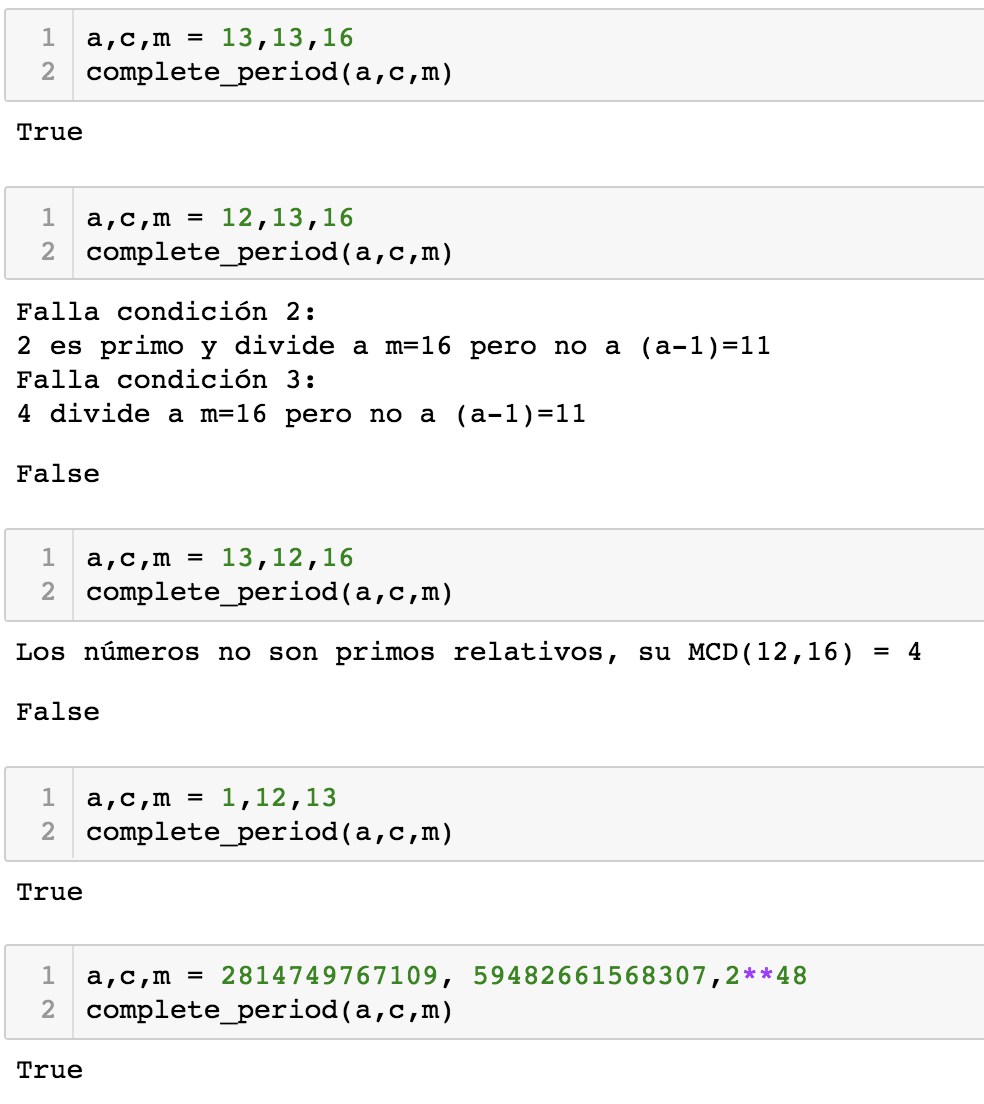
\includegraphics[width=11.5cm]{output_3.png}
    \end{figure}
    
    \newpage
    
    
    \item Mostrar que el promedio de las $U_i’s$ tomadas de un ciclo completo de un GLC de periodo completo es $\frac{1}{2} - \frac{1}{m} $
    
    \underline{Demostración:}
    
    Notemos que dado un generador de ciclo completo, si $Z_i \equiv$ $\left[a^iZ_0 + c\frac{a^i - 1}{a - 1}\right] mod \ m$ entonces $\{ Z_i \ | \ 0 \leq i < m, \} = \{0,1,...,m-1\}$. 
    
    Para probar dicha afirmación basta notar que por un lado $\{ Z_i \ | \ 0 \leq i < m, \} \subset \{0,1,...,m-1\}$ por la definición de los $Z_i's$. Por otro lado $\{0,1,...,m-1\} \subset \{ Z_i \ | \ 0 \leq i < m, \} $ pues en caso contrario el generador no sería completo. 
    
    Con dicha observación, tenemos: 
    \begin{align*}
        \frac{1}{m}\sum_{i=1}^{m} U_i &= \frac{1}{m}\sum_{i=1}^{m} \frac{Z_i}{m} \\
        &= \frac{1}{m^2}\sum_{i=1}^{m}  Z_i  \\
        &= \frac{1}{m^2}\sum_{i\in\mathbb{N}, i<m} i \\
        &= \frac{1}{m^2} \frac{(m-1)(m)}{2} \\
        &= \frac{(m-1)}{2m} \\
        &= \frac{m}{2} - \frac{1}{2m}
    \end{align*}
    \qedsymbol
    
    \newpage
    
    \item Generar 10,000 números con U (0, 1) de Excel. Hacer un breve estudio para probar la calidad de los generadores; aplicar las pruebas de uniformidad e independencia a cada conjunto de datos. Resumir resultados en NO MAS de 2 cuartillas, incluyendo gráficas. De acuerdo a tus resultados, ¿cómo calificarías al generador de Excel?
    
    \newpage
    \item Probar que la parte fraccional de la suma de uniformes en $[0,1]$: $U_1 + U_2 + ... + U_k$ es también uniforme en el intervalo $[0,1]$.
    
    \underline{Demostración:} 
    
    Comencemos por notar que, dadas $U_1$ y $U_2$ variables aleatorias con distribución uniforme, entonces la parte fraccional de $U_1 + U_2$ tiene dicha distribución.
    
    Denotemos por $\{x\} = x -  \lceil x \rceil $ la parte fraccional de x, sabmemos que la densidad de $U = U_1 + U_2$ es la siguiente: 
    \begin{align*}
        f_U(x) = \begin{cases} 
              x & 0 \leq x \leq 1\\
              2-x & 1 < x \leq 2
           \end{cases}
    \end{align*}
    
    Asimismo, la distribución de $\{U\} = \{U_1 + U_2\}$ está dada por:
    \begin{align*}
        F_{\{U\}}(u) &= P\{ \{U\} <= u\} \\
        &= P\{ U - \lfloor U \rfloor <= u\} \\
        &= P\{ U <= u,\ 0 \leq U \leq 1 \} + P\{ U - \lfloor U \rfloor <= u,\ 1 < U \leq 2 \} \\
        &= \int_0^u f_U(x) dx + \int_1^{1+u} f_U(x) dx \\
        &= \int_0^u x dx + \int_1^{1+u} 2-x dx\\
        &= \frac{u^2}{2} + 2u - \frac{(1+u)^2}{2} + \frac{1}{2}\\
        &= u
    \end{align*}
    
    De esta manera la parte fraccional de $U_1 + U_2$ tiene distribución uniforme en el intervalo $(0,1)$. 
    
    Para la prueba del caso general $U_1 + ... + U_k$ se debe proceder por inducción; si se supone que la parte fraccional de la suma de $n-1$ variables aleatorias con distrución uniforme sigue dicha distrución, es suficiente notar que $\{U_1 + U_2 +... + U_k\} =\{\{U_1\} + \{U_2 + ... + U_k\}\}$ para concluir con la demostración.

    \qedsymbol
    
    
    \newpage
    
    \item Un generador de Fibonacci obtiene Xn+1 a partir de Xn y Xn−1 de la siguiente forma:
    
    \begin{align*}
        X_{i+1} = (X_i + X_{i-1}) \ mod \ m
    \end{align*}
    
    Con $X_0$ y $X_1$ dados. Para $m=5$ solo dos ciclos son posibles, encontrarlos y al periodo.
    
    \underline{Solucion:}
    
    Para la solución a dicho problema se implementaron las siguientes funciones en python3
    
    \inputminted[fontsize=\scriptsize]{python}{fibonacci_generator.py}
    
    La función \underline{fibo} recibe como parámetros $X_0$ y $X_1$, las raíces y m, el módulo. Y genera el los números producidos por la iteración hasta caer en un ciclo, como ejemplos:
    
    \begin{figure}[h]
        \centering
        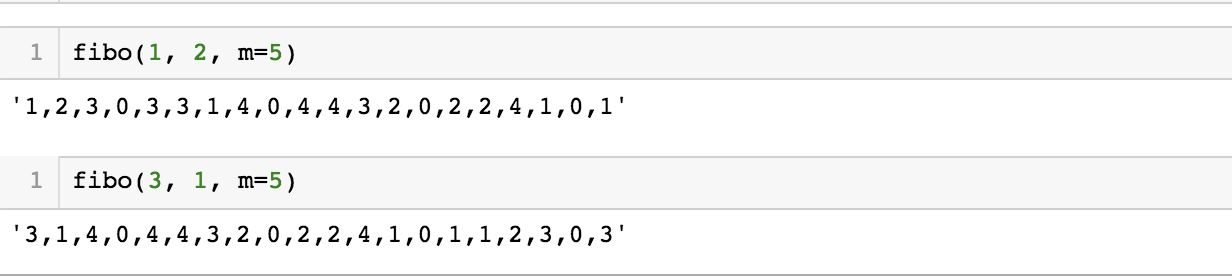
\includegraphics[width=11cm]{fibonacci.png}
    \end{figure}
    
    Haciendo uso de dicha función, la siguiente función obtiene todos los posibles ciclos de el generador de fibonacci para un n dado, para $n=5$ tenemos los siguientes resultados:
    
    \begin{figure}[h]
        \centering
        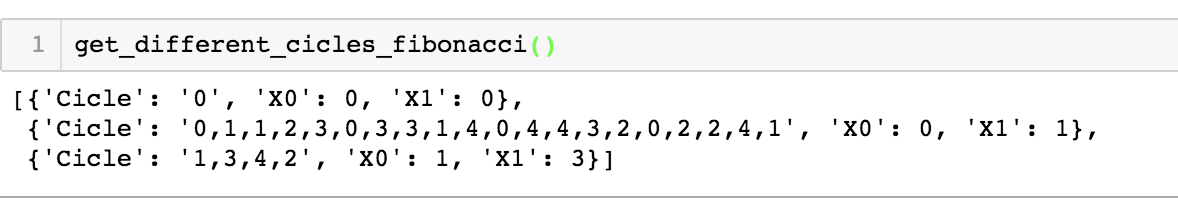
\includegraphics[width=11cm]{cicles.png}
    \end{figure}
    
    Notamos que, además del ciclo trivial, hay 2 ciclos distintos.
    
    \newpage
    
    \item Genera 10,000 números con una semilla de $Z_0 = 1$ usando el generador $Z_n = 75Z_{n-1} \ mod  \ (2^{31} −1)$ Clasifica los números en 10 celdas de igual tamaño y prueben por  uniformidad usando la prueba $\chi^2$ con un nivel de confianza del 90\%. Aplicar también la prueba de rachas.
    
    \underline{Solución}

\begin{knitrout}
\definecolor{shadecolor}{rgb}{0.969, 0.969, 0.969}\color{fgcolor}\begin{kframe}
\begin{alltt}
\hlkwd{library}\hlstd{(tidyverse)}
\hlkwd{library}\hlstd{(randtests)}
\end{alltt}
\end{kframe}
\end{knitrout}

\begin{knitrout}
\definecolor{shadecolor}{rgb}{0.969, 0.969, 0.969}\color{fgcolor}\begin{kframe}
\begin{alltt}
\hlstd{GLC} \hlkwb{=} \hlkwa{function}\hlstd{(}\hlkwc{z0}\hlstd{,}\hlkwc{a}\hlstd{,}\hlkwc{c}\hlstd{,}\hlkwc{m}\hlstd{,}\hlkwc{k}\hlstd{)\{}
    \hlstd{Ui} \hlkwb{=} \hlkwd{rep}\hlstd{(}\hlnum{0}\hlstd{,k)}
    \hlstd{Ui[}\hlnum{1}\hlstd{]} \hlkwb{=} \hlstd{z0}\hlopt{/}\hlstd{m}
    \hlstd{z} \hlkwb{=} \hlstd{(z0}\hlopt{*}\hlstd{a} \hlopt{+} \hlstd{c)}\hlopt\hlstd{m}
    \hlkwa{for} \hlstd{(i} \hlkwa{in} \hlnum{2}\hlopt{:}\hlstd{k)\{}
        \hlstd{Ui[i]} \hlkwb{=} \hlstd{z}\hlopt{/}\hlstd{m}
        \hlstd{z} \hlkwb{=} \hlstd{(z}\hlopt{*}\hlstd{a} \hlopt{+} \hlstd{c)}\hlopt\hlstd{m}
    \hlstd{\}}
    \hlkwd{return} \hlstd{(}\hlkwd{as.data.frame}\hlstd{(Ui))}
\hlstd{\}}

\hlstd{df} \hlkwb{=} \hlkwd{GLC}\hlstd{(}\hlnum{1}\hlstd{,}\hlnum{7}\hlopt{^}\hlnum{5}\hlstd{,}\hlnum{0}\hlstd{,}\hlnum{2}\hlopt{^}\hlnum{31}\hlopt{-}\hlnum{1}\hlstd{,}\hlnum{10000}\hlstd{)}
\hlstd{unif} \hlkwb{=} \hlstd{df}\hlopt{$}\hlstd{Ui}

\hlstd{h} \hlkwb{=} \hlkwd{hist}\hlstd{(unif,} \hlkwc{breaks} \hlstd{=} \hlnum{10}\hlstd{,} \hlkwc{right} \hlstd{=} \hlnum{FALSE}\hlstd{,} \hlkwc{plot} \hlstd{=} \hlnum{FALSE}\hlstd{)}
\hlstd{breaks_cdf} \hlkwb{<-} \hlkwd{punif}\hlstd{(h}\hlopt{$}\hlstd{breaks)}
\hlstd{null.probs} \hlkwb{<-} \hlstd{breaks_cdf[}\hlopt{-}\hlnum{1}\hlstd{]} \hlopt{-} \hlstd{breaks_cdf[}\hlopt{-}\hlkwd{length}\hlstd{(breaks_cdf)]}
\hlkwd{print}\hlstd{(}\hlkwd{chisq.test}\hlstd{(h}\hlopt{$}\hlstd{counts,} \hlkwc{p} \hlstd{= null.probs,} \hlkwc{rescale.p} \hlstd{= T))}
\end{alltt}
\begin{verbatim}
## 
## 	Chi-squared test for given probabilities
## 
## data:  h$counts
## X-squared = 6.676, df = 9, p-value = 0.6708
\end{verbatim}
\end{kframe}
\end{knitrout}
Concluimos con un nivel de significancia del 90\%, dado que el valor p es mayor que .1, que los números generados siguen una distribución uniforme.

Ahora apliquemos la prueba de rachas, por default la función runs.test del paquete \textit{randtests} de R realiza la prueba de rachas de \textit{Wald-Wolfowitz}.

\begin{knitrout}
\definecolor{shadecolor}{rgb}{0.969, 0.969, 0.969}\color{fgcolor}\begin{kframe}
\begin{alltt}
\hlkwd{runs.test}\hlstd{(unif,} \hlkwc{plot} \hlstd{= T)}
\end{alltt}
\end{kframe}
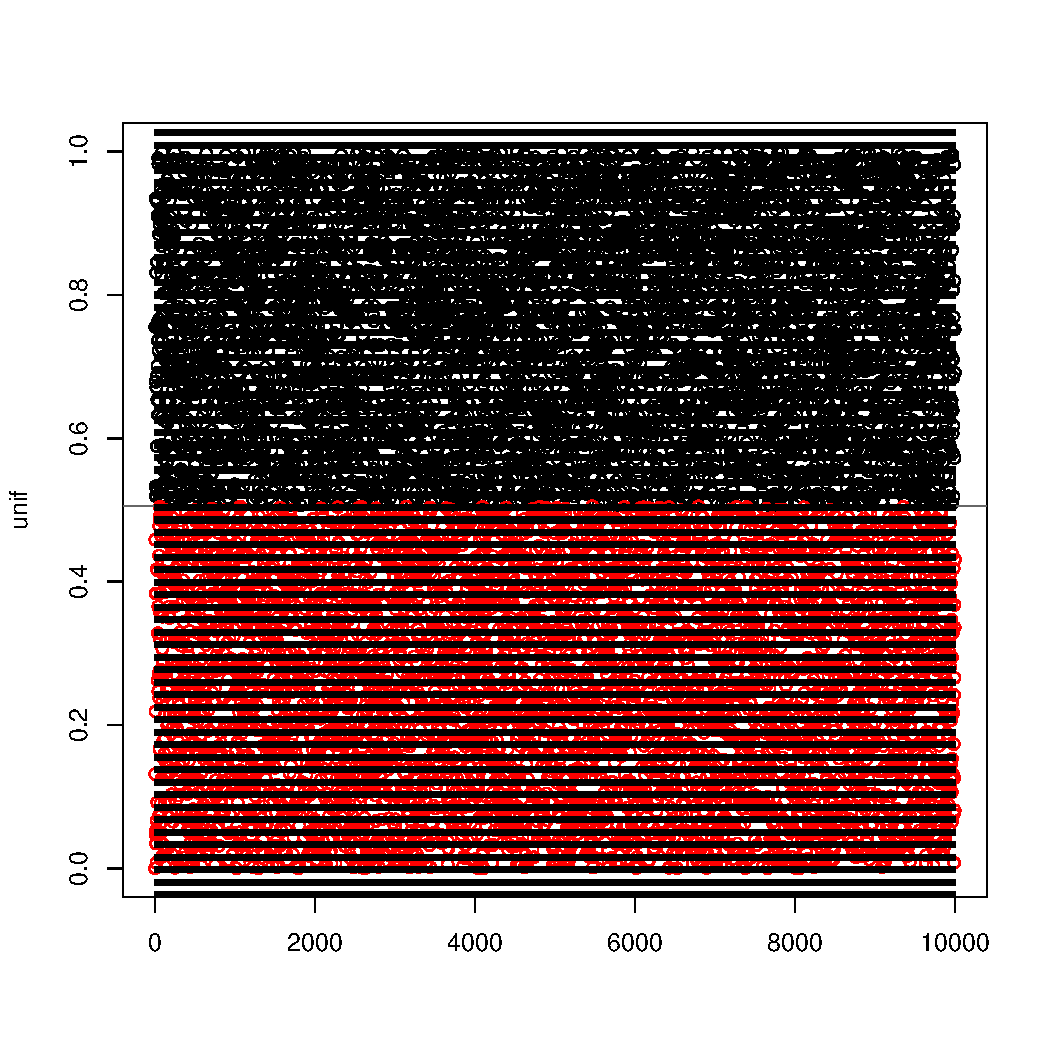
\includegraphics[width=\maxwidth]{figure/unnamed-chunk-4-1} 
\begin{kframe}\begin{verbatim}
## 
## 	Runs Test
## 
## data:  unif
## statistic = -1.1801, runs = 4942, n1 = 5000, n2 = 5000, n = 10000,
## p-value = 0.238
## alternative hypothesis: nonrandomness
\end{verbatim}
\end{kframe}
\end{knitrout}

Notamos que no hay argumentos para rechazar la hipótesis alterntativa de no aleatoriedad puesto que el p-value es mayor que .1.


\newpage

\item Aplicar a los datos del ejercicio las pruebas de correlación, gaps y poker.

Comencemos por aplicar la prueba de poker, por default las \textit{manos} son de tamaño 5.

\begin{knitrout}
\definecolor{shadecolor}{rgb}{0.969, 0.969, 0.969}\color{fgcolor}\begin{kframe}
\begin{alltt}
\hlkwd{library}\hlstd{(randtoolbox)}
\end{alltt}


{\ttfamily\noindent\itshape\color{messagecolor}{\#\# Loading required package: rngWELL}}

{\ttfamily\noindent\itshape\color{messagecolor}{\#\# This is randtoolbox. For overview, type 'help("{}randtoolbox"{})'.}}

{\ttfamily\noindent\itshape\color{messagecolor}{\#\# \\\#\# Attaching package: 'randtoolbox'}}

{\ttfamily\noindent\itshape\color{messagecolor}{\#\# The following object is masked from 'package:randtests':\\\#\# \\\#\#\ \ \ \  permut}}\begin{alltt}
\hlkwd{poker.test}\hlstd{(unif)}
\end{alltt}
\begin{verbatim}
## 
## 			 Poker test
## 
## chisq stat = 1.4, df = 4, p-value = 0.85
## 
## 		 (sample size : 10000)
## 
## 	observed number	 3 204 956 755 82 
## 	expected number	 3.2 192 960 768 77
\end{verbatim}
\end{kframe}
\end{knitrout}

La prueba de poker no presenta argumento para rechazar la hipótesis de no aleatoriedad puesto que se reporta un p-value = .85.

Ahora realicemos la prueba de gaps. Por default, la función \textit{gap.test} de R considera como gap al intervalo [0,.5], realizando la prueba obtenemos:

\begin{knitrout}
\definecolor{shadecolor}{rgb}{0.969, 0.969, 0.969}\color{fgcolor}\begin{kframe}
\begin{alltt}
\hlkwd{gap.test}\hlstd{(unif)}
\end{alltt}
\begin{verbatim}
## 
## 			 Gap test
## 
## chisq stat = 7.6, df = 13, p-value = 0.87
## 
## 		 (sample size : 10000)
## 
## length	observed freq		theoretical freq
## 1 			 1207 			 1250 
## 2 			 642 			 625 
## 3 			 313 			 312 
## 4 			 161 			 156 
## 5 			 70 			 78 
## 6 			 34 			 39 
## 7 			 22 			 20 
## 8 			 12 			 9.8 
## 9 			 5 			 4.9 
## 10 			 1 			 2.4 
## 11 			 1 			 1.2 
## 12 			 0 			 0.61 
## 13 			 1 			 0.31 
## 14 			 0 			 0.15
\end{verbatim}
\end{kframe}
\end{knitrout}

Observamos que el p-value es igual a .87 de forma que no tenemos argumentos para rechazar la hipótesis de no aleatoriedad. Sin embargo, realizaremos la prueba de gaps una vez más pero ahora moficicando el intervalo a [.3,.6]

\begin{knitrout}
\definecolor{shadecolor}{rgb}{0.969, 0.969, 0.969}\color{fgcolor}\begin{kframe}
\begin{alltt}
\hlkwd{gap.test}\hlstd{(unif,} \hlkwc{lower} \hlstd{=} \hlnum{.3}\hlstd{,} \hlkwc{upper} \hlstd{=} \hlnum{.6}\hlstd{)}
\end{alltt}
\begin{verbatim}
## 
## 			 Gap test
## 
## chisq stat = 15, df = 7, p-value = 0.037
## 
## 		 (sample size : 10000)
## 
## length	observed freq		theoretical freq
## 1 			 1498 			 1470 
## 2 			 418 			 441 
## 3 			 138 			 132 
## 4 			 35 			 40 
## 5 			 17 			 12 
## 6 			 1 			 3.6 
## 7 			 4 			 1.1 
## 8 			 0 			 0.32
\end{verbatim}
\end{kframe}
\end{knitrout}

Observamos que el p-value es igual a 0.037 de forma que rechazamos la hipótesis de aleatoriedad.

Finalmente, realizaremos la prueba de autocorrelación. Para ello se obtendrá la función de autocorrelación utilizando el paquete \textit{forecast}.

\begin{knitrout}
\definecolor{shadecolor}{rgb}{0.969, 0.969, 0.969}\color{fgcolor}\begin{kframe}
\begin{alltt}
\hlkwd{library}\hlstd{(hwwntest)}
\hlkwd{library}\hlstd{(forecast)}

\hlcom{#Obteniendo la función de autocorrelación}
\hlstd{ACF} \hlkwb{=} \hlkwd{Acf}\hlstd{(unif)}
\end{alltt}
\end{kframe}
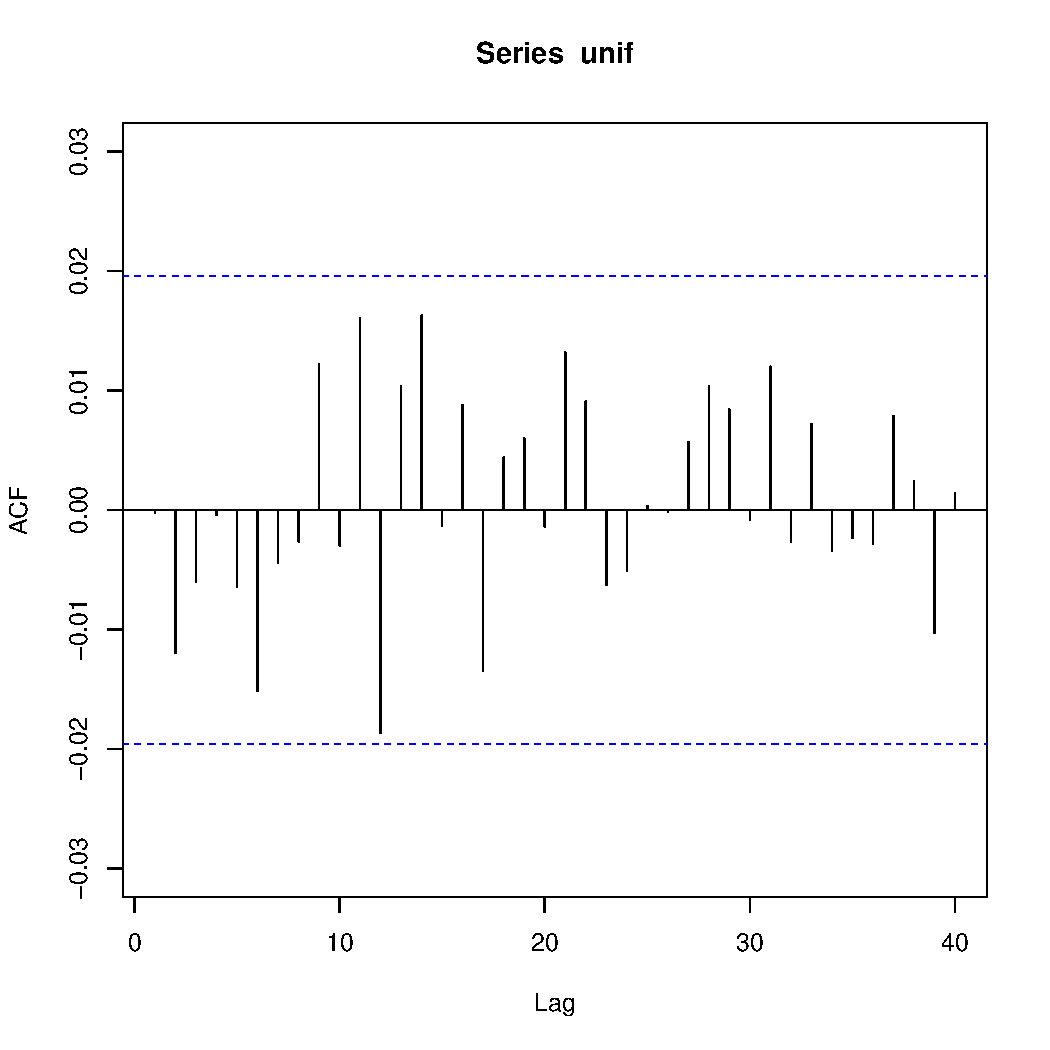
\includegraphics[width=\maxwidth]{figure/unnamed-chunk-8-1} 
\begin{kframe}\begin{alltt}
\hlcom{#Realizando el test de Bartlett}
\hlstd{rho} \hlkwb{<-} \hlstd{ACF}\hlopt{$}\hlstd{acf[}\hlnum{2}\hlstd{]}
\hlstd{bt} \hlkwb{<-} \hlkwd{sqrt}\hlstd{(}\hlkwd{length}\hlstd{(unif))}\hlopt{*}\hlstd{rho}
\hlstd{p.value} \hlkwb{=} \hlnum{1}\hlopt{-}\hlkwd{pnorm}\hlstd{(bt)}\hlopt{/}\hlnum{2}
\hlkwd{print}\hlstd{(p.value)}
\end{alltt}
\begin{verbatim}
## [1] 0.75
\end{verbatim}
\begin{alltt}
\hlcom{#Test de Bartlett para ruido blanco}
\hlkwd{bartlettB.test}\hlstd{(unif)}
\end{alltt}
\begin{verbatim}
## 
## 	Bartlett B Test for white noise
## 
## data:  
## = 0.6, p-value = 0.9
\end{verbatim}
\begin{alltt}
\hlcom{#Test de Box-Pierce}
\hlkwd{Box.test}\hlstd{(unif,}\hlkwc{lag}\hlstd{=}\hlnum{5}\hlstd{,}\hlkwc{type}\hlstd{=}\hlstr{"Box-Pierce"}\hlstd{)}
\end{alltt}
\begin{verbatim}
## 
## 	Box-Pierce test
## 
## data:  unif
## X-squared = 2, df = 5, p-value = 0.8
\end{verbatim}
\begin{alltt}
\hlcom{#Test de Ljung-Box}
\hlkwd{Box.test}\hlstd{(unif,}\hlkwc{lag}\hlstd{=}\hlnum{5}\hlstd{,}\hlkwc{type}\hlstd{=}\hlstr{"Ljung-Box"}\hlstd{)}
\end{alltt}
\begin{verbatim}
## 
## 	Box-Ljung test
## 
## data:  unif
## X-squared = 2, df = 5, p-value = 0.8
\end{verbatim}
\end{kframe}
\end{knitrout}

Como se muestra en la gráfica, la función de autocorrelación no presenta valores extremos, asimismo, ninguna prueba de autocorrelación presenta argumentos para rechazar la hipótesis de aleatoriedad.
    
\newpage

\item Generar 1500 números del generador RANDU. Hacer una prueba de Kolmogorov-Smirnov al 95\% de confianza.


\underline{Solución}:

A continuación se realizara la prueba de Kolmogov-Smirnof a los dígitos generados por el generador RANDU con dos semillas distintas, 100 y 32.

\begin{knitrout}
\definecolor{shadecolor}{rgb}{0.969, 0.969, 0.969}\color{fgcolor}\begin{kframe}
\begin{alltt}
\hlstd{randu1} \hlkwb{=} \hlkwd{GLC}\hlstd{(}\hlnum{100}\hlstd{,}\hlnum{2}\hlopt{^}\hlnum{16} \hlopt{+}\hlnum{3}\hlstd{,}\hlnum{0}\hlstd{,} \hlnum{2}\hlopt{^}\hlnum{31}\hlstd{,}\hlnum{1500}\hlstd{)}
\hlkwd{print}\hlstd{(}\hlkwd{ks.test}\hlstd{(randu1}\hlopt{$}\hlstd{Ui,}\hlstr{"punif"}\hlstd{))}
\end{alltt}
\begin{verbatim}
## 
## 	One-sample Kolmogorov-Smirnov test
## 
## data:  randu1$Ui
## D = 0.01, p-value = 0.9
## alternative hypothesis: two-sided
\end{verbatim}
\begin{alltt}
\hlstd{randu2} \hlkwb{=} \hlkwd{GLC}\hlstd{(}\hlnum{32}\hlstd{,}\hlnum{2}\hlopt{^}\hlnum{16} \hlopt{+}\hlnum{3}\hlstd{,}\hlnum{0}\hlstd{,} \hlnum{2}\hlopt{^}\hlnum{31}\hlstd{,}\hlnum{1500}\hlstd{)}
\hlkwd{print}\hlstd{(} \hlkwd{ks.test}\hlstd{(randu2}\hlopt{$}\hlstd{Ui,}\hlstr{"punif"}\hlstd{) )}
\end{alltt}
\begin{verbatim}
## 
## 	One-sample Kolmogorov-Smirnov test
## 
## data:  randu2$Ui
## D = 0.04, p-value = 0.01
## alternative hypothesis: two-sided
\end{verbatim}
\end{kframe}
\end{knitrout}

Los resultados arrojados por la prueba a un nivel del 95\% de confianza no presentan argumentos para rechazar la hipótesis nula (de uniformidad) en el primer caso (semilla $X_0=100$) puesto que le valor p es igual a .9351. 

Asimismo, en el segundo caso ($X_0 = 32$) se rechaza la hipótesis nula puesto que el valor p es .01358.

\newpage

\item La página The number e to one million digits  contiene el primer millón de
dígitos de e (pueden usar cualquier otra página). Considerando estos dígitos:

\begin{itemize}
    \item Realizar un histograma y verificar la hipótesis de que los dígitos corresponden a una distribución uniforme discreta.
    
    \item Verificar independencia de los dígitos, considerando las pruebas de gaps, de poker y de rachas. Una idea de ver los datos está en la siguiente imagen (esta está hecha para $\pi$):
    
\end{itemize}

Comenzamos con la lectura de los dígitos:

\begin{knitrout}
\definecolor{shadecolor}{rgb}{0.969, 0.969, 0.969}\color{fgcolor}\begin{kframe}
\begin{alltt}
\hlstd{decimals_e} \hlkwb{=} \hlkwd{readChar}\hlstd{(}\hlstr{'e.txt'}\hlstd{,} \hlkwd{file.info}\hlstd{(}\hlstr{'e.txt'}\hlstd{)}\hlopt{$}\hlstd{size)}
\end{alltt}


{\ttfamily\noindent\color{warningcolor}{\#\# Warning in file(con, "{}rb"{}): no fue posible abrir el archivo 'e.txt': No such file or directory}}

{\ttfamily\noindent\bfseries\color{errorcolor}{\#\# Error in file(con, "{}rb"{}): no se puede abrir la conexión}}\begin{alltt}
\hlstd{decimals_e} \hlkwb{=} \hlkwd{gsub}\hlstd{(}\hlstr{'\textbackslash{}n'}\hlstd{,} \hlstr{''}\hlstd{, decimals_e)}
\end{alltt}


{\ttfamily\noindent\bfseries\color{errorcolor}{\#\# Error in gsub("{}\textbackslash{}n"{}, "{}"{}, decimals\_e): objeto 'decimals\_e' no encontrado}}\begin{alltt}
\hlstd{df} \hlkwb{=} \hlkwd{data.frame}\hlstd{(}\hlstr{"val"} \hlstd{=} \hlkwd{unlist}\hlstd{((}\hlkwd{strsplit}\hlstd{(decimals_e,} \hlstr{''}\hlstd{))))}
\end{alltt}


{\ttfamily\noindent\bfseries\color{errorcolor}{\#\# Error in strsplit(decimals\_e, "{}"{}): objeto 'decimals\_e' no encontrado}}\begin{alltt}
\hlstd{df}\hlopt{$}\hlstd{val} \hlkwb{=} \hlkwd{as.numeric}\hlstd{(}\hlkwd{as.character}\hlstd{(df}\hlopt{$}\hlstd{val))}
\end{alltt}


{\ttfamily\noindent\bfseries\color{errorcolor}{\#\# Error in `\$<-.data.frame`(`*tmp*`, val, value = numeric(0)): replacement has 0 rows, data has 10000}}\end{kframe}
\end{knitrout}

Realizamos un histograma de los mismos:

\begin{knitrout}
\definecolor{shadecolor}{rgb}{0.969, 0.969, 0.969}\color{fgcolor}\begin{kframe}
\begin{alltt}
\hlkwd{ggplot}\hlstd{(df,} \hlkwd{aes}\hlstd{(val))} \hlopt{+}
    \hlkwd{geom_histogram}\hlstd{(}\hlkwc{breaks} \hlstd{=} \hlkwd{seq}\hlstd{(}\hlopt{-}\hlnum{.5}\hlstd{,}\hlnum{9.5}\hlstd{,}\hlkwc{by} \hlstd{=} \hlnum{1}\hlstd{))} \hlopt{+}
    \hlkwd{labs}\hlstd{(}\hlkwc{title}\hlstd{=}\hlstr{"Histograma de primer millón de dígitos de e"}\hlstd{,}
    \hlkwc{y}\hlstd{=}\hlstr{"Frecuencia"}\hlstd{,} \hlkwc{x}\hlstd{=}\hlstr{"Dígito"}\hlstd{)}
\end{alltt}


{\ttfamily\noindent\bfseries\color{errorcolor}{\#\# Error in FUN(X[[i]], ...): objeto 'val' no encontrado}}\end{kframe}

\includegraphics[width=\maxwidth]{figure/unnamed-chunk-11-1} 

\end{knitrout}

Realizamos una serie de gráficas qq-plot 

\begin{knitrout}
\definecolor{shadecolor}{rgb}{0.969, 0.969, 0.969}\color{fgcolor}\begin{kframe}
\begin{alltt}
\hlstd{graf.teorica} \hlkwb{<-} \hlkwa{function}\hlstd{(}\hlkwc{fun.quan}\hlstd{,}\hlkwc{x}\hlstd{,}\hlkwc{tit}\hlstd{,}\hlkwc{...}\hlstd{)\{}
    \hlstd{z} \hlkwb{<-} \hlkwd{sort}\hlstd{(x,}\hlkwc{decreasing}\hlstd{=F)}
    \hlkwd{plot}\hlstd{(}\hlkwd{fun.quan}\hlstd{(}\hlkwd{ppoints}\hlstd{(z),}\hlnum{0}\hlstd{,}\hlnum{10}\hlstd{),z,}\hlkwc{main}\hlstd{=tit,}\hlkwc{xlab} \hlstd{=}
    \hlstr{"dist. teorica"}\hlstd{,}\hlkwc{ylab} \hlstd{=} \hlstr{"datos"}\hlstd{)}
    \hlkwd{abline}\hlstd{(}\hlkwc{a}\hlstd{=}\hlnum{0}\hlstd{,}\hlkwc{b}\hlstd{=}\hlnum{1}\hlstd{)}
\hlstd{\}}

\hlkwd{par}\hlstd{(}\hlkwc{mfrow} \hlstd{=} \hlkwd{c}\hlstd{(}\hlnum{2}\hlstd{,}\hlnum{2}\hlstd{))}

\hlkwd{graf.teorica}\hlstd{(qunif,} \hlkwd{head}\hlstd{(df}\hlopt{$}\hlstd{val,}\hlnum{20}\hlstd{),} \hlkwc{tit} \hlstd{=} \hlstr{"20 dígitos"}\hlstd{)}
\end{alltt}


{\ttfamily\noindent\bfseries\color{errorcolor}{\#\# Error in if (n > 0) (1L:n - a)/(n + 1 - 2 * a) else numeric(): argumento tiene longitud cero}}\begin{alltt}
\hlkwd{graf.teorica}\hlstd{(qunif,} \hlkwd{head}\hlstd{(df}\hlopt{$}\hlstd{val,}\hlnum{50}\hlstd{),} \hlkwc{tit} \hlstd{=} \hlstr{"50 dígitos"}\hlstd{)}
\end{alltt}


{\ttfamily\noindent\bfseries\color{errorcolor}{\#\# Error in if (n > 0) (1L:n - a)/(n + 1 - 2 * a) else numeric(): argumento tiene longitud cero}}\begin{alltt}
\hlkwd{graf.teorica}\hlstd{(qunif,} \hlkwd{head}\hlstd{(df}\hlopt{$}\hlstd{val,}\hlnum{125}\hlstd{),} \hlkwc{tit} \hlstd{=} \hlstr{"125 dígitos"}\hlstd{)}
\end{alltt}


{\ttfamily\noindent\bfseries\color{errorcolor}{\#\# Error in if (n > 0) (1L:n - a)/(n + 1 - 2 * a) else numeric(): argumento tiene longitud cero}}\begin{alltt}
\hlkwd{graf.teorica}\hlstd{(qunif,} \hlkwd{head}\hlstd{(df}\hlopt{$}\hlstd{val,}\hlnum{10000}\hlstd{),} \hlkwc{tit} \hlstd{=} \hlstr{"10000 dígitos"}\hlstd{)}
\end{alltt}


{\ttfamily\noindent\bfseries\color{errorcolor}{\#\# Error in if (n > 0) (1L:n - a)/(n + 1 - 2 * a) else numeric(): argumento tiene longitud cero}}\end{kframe}
\end{knitrout}
El test de $\chi^2$ a un nivel de 95\% de confianza:

\begin{knitrout}
\definecolor{shadecolor}{rgb}{0.969, 0.969, 0.969}\color{fgcolor}\begin{kframe}
\begin{alltt}
\hlstd{punifdisc} \hlkwb{<-} \hlkwa{function}\hlstd{(}\hlkwc{q}\hlstd{,} \hlkwc{min}\hlstd{=}\hlnum{0}\hlstd{,} \hlkwc{max}\hlstd{=}\hlnum{9}\hlstd{)} \hlkwd{ifelse}\hlstd{(q}\hlopt{<}\hlstd{min,}
\hlnum{0}\hlstd{,} \hlkwd{ifelse}\hlstd{(q}\hlopt{>=}\hlstd{max,} \hlnum{1}\hlstd{, (}\hlkwd{floor}\hlstd{(q)}\hlopt{-}\hlstd{min}\hlopt{+}\hlnum{1}\hlstd{)}\hlopt{/}\hlstd{(max}\hlopt{-}\hlstd{min}\hlopt{+}\hlnum{1}\hlstd{)))}
\hlstd{qunifdisc} \hlkwb{<-} \hlkwa{function}\hlstd{(}\hlkwc{p}\hlstd{,} \hlkwc{min}\hlstd{=}\hlnum{0}\hlstd{,} \hlkwc{max}\hlstd{=}\hlnum{9}\hlstd{)} \hlkwd{floor}\hlstd{(p}\hlopt{*}\hlstd{(max}\hlopt{-}\hlstd{min}\hlopt{+}\hlnum{1}\hlstd{))}

\hlstd{h1} \hlkwb{<-} \hlkwd{hist}\hlstd{(df}\hlopt{$}\hlstd{val,} \hlkwc{breaks} \hlstd{=} \hlkwd{seq}\hlstd{(}\hlopt{-}\hlnum{.5}\hlstd{,}\hlnum{9.5}\hlstd{,}\hlkwc{by} \hlstd{=} \hlnum{1}\hlstd{),} \hlkwc{plot} \hlstd{= F)}
\end{alltt}


{\ttfamily\noindent\bfseries\color{errorcolor}{\#\# Error in hist.default(df\$val, breaks = seq(-0.5, 9.5, by = 1), plot = F): 'x' must be numeric}}\begin{alltt}
\hlstd{breaks_cdf} \hlkwb{<-} \hlkwd{punifdisc}\hlstd{(h1}\hlopt{$}\hlstd{breaks)}
\end{alltt}


{\ttfamily\noindent\bfseries\color{errorcolor}{\#\# Error in ifelse(q < min, 0, ifelse(q >= max, 1, (floor(q) - min + 1)/(max - : objeto 'h1' no encontrado}}\begin{alltt}
\hlstd{null.probs} \hlkwb{<-} \hlstd{breaks_cdf[}\hlopt{-}\hlnum{1}\hlstd{]} \hlopt{-} \hlstd{breaks_cdf[}\hlopt{-}\hlkwd{length}\hlstd{(breaks_cdf)]}
\hlstd{a} \hlkwb{<-} \hlkwd{chisq.test}\hlstd{(h1}\hlopt{$}\hlstd{counts,} \hlkwc{p} \hlstd{= null.probs,} \hlkwc{rescale.p} \hlstd{= T)}
\end{alltt}


{\ttfamily\noindent\bfseries\color{errorcolor}{\#\# Error in is.data.frame(x): objeto 'h1' no encontrado}}\begin{alltt}
\hlstd{a}
\end{alltt}


{\ttfamily\noindent\bfseries\color{errorcolor}{\#\# Error in eval(expr, envir, enclos): objeto 'a' no encontrado}}\end{kframe}
\end{knitrout}

Dado que el valor p es mayor que .05 no existen argumentos para rechazar la hipótesis de uniformidad. Continuemos con las pruebas de independencia.

\begin{knitrout}
\definecolor{shadecolor}{rgb}{0.969, 0.969, 0.969}\color{fgcolor}\begin{kframe}
\begin{alltt}
\hlkwd{runs.test}\hlstd{(unif)}
\end{alltt}
\begin{verbatim}
## 
## 	Runs Test
## 
## data:  unif
## statistic = -1, runs = 5000, n1 = 5000, n2 = 5000, n = 10000,
## p-value = 0.2
## alternative hypothesis: nonrandomness
\end{verbatim}
\begin{alltt}
\hlcom{#poker.test(unif)}
\hlcom{#gap.test(unif)}
\end{alltt}
\end{kframe}
\end{knitrout}



\end{enumerate}



\end{document}
